\documentclass{beamer}

\usepackage{helvet}
\usepackage{hyperref, graphicx}
\usepackage{amsthm}
\usepackage{etoolbox}
\usepackage{multicol}
\usepackage{tikz}
\usepackage{ulem}

\usetheme{default}
\setbeamertemplate{navigation symbols}{}
\AtBeginSection[ ]
{
\begin{frame}{Outline}
    \tableofcontents[currentsection]
\end{frame}
}

% Default fixed font does not support bold face
\DeclareFixedFont{\ttb}{T1}{txtt}{bx}{n}{11} % for bold
\DeclareFixedFont{\ttm}{T1}{txtt}{m}{n}{12}  % for normal - use in headings

% Custom colors
\usepackage{color}
\definecolor{TUGray}{RGB}{101,101,137}
\definecolor{TUBlack}{RGB}{30,0,0}
\definecolor{mygreen}{RGB}{45,111,63}
\definecolor{keywords}{RGB}{205,114,0}
\definecolor{comments}{RGB}{181,51,139}
\definecolor{strings}{RGB}{58,144,81}
\definecolor{numeric}{RGB}{66,110,176}
\definecolor{linos}{rgb}{0.4,0.4,0.4}
\definecolor{links}{rgb}{0,0.4,0.75}

\definecolor{bggray}{RGB}{232, 233, 235}

\usecolortheme[named=mygreen]{structure}
\setbeamercolor{normal text}{fg=TUBlack}\usebeamercolor*{normal text}

\setbeamercolor{codecol}{fg=TUGray!25!black,bg=bggray}

\hypersetup{colorlinks, linkcolor=links, urlcolor=links}

\usepackage[T1]{fontenc}
\usepackage[sfdefault,scaled=.85]{FiraSans}
\usepackage{newtxsf}

\usepackage{listings}

\newtoggle{InString}{}% Keep track of if we are within a string
\togglefalse{InString}% Assume not initally in string

\newcommand\digitstyle{\color{numeric}}
\makeatletter
\newcommand{\ProcessDigit}[1]
{%
  \ifnum\lst@mode=\lst@Pmode\relax%
   {\digitstyle #1}%
  \else
    #1%
  \fi
}
\makeatother

\lstset{literate=%
    {0}{{{\ProcessDigit{0}}}}1
    {1}{{{\ProcessDigit{1}}}}1
    {2}{{{\ProcessDigit{2}}}}1
    {3}{{{\ProcessDigit{3}}}}1
    {4}{{{\ProcessDigit{4}}}}1
    {5}{{{\ProcessDigit{5}}}}1
    {6}{{{\ProcessDigit{6}}}}1
    {7}{{{\ProcessDigit{7}}}}1
    {8}{{{\ProcessDigit{8}}}}1
    {9}{{{\ProcessDigit{9}}}}1
	{<=}{{\(\leq\)}}1
	{>=}{{\(\geq\)}}1,
	% morestring=[b]",
    % morestring=[b]',
    % morecomment=[l]{//},
}

\lstdefinelanguage{Pseudo}{
    morekeywords={return, while, if, for, input},
    morecomment=[l]{\#},
}

% Pseudocode style
\newcommand\pseudostyle{\lstset{
language=Pseudo,
basicstyle=\fontfamily{ccr}\scriptsize,
commentstyle=\it\scriptsize\color{linos},
keywordstyle=\it\bfseries\scriptsize,
mathescape=true,
literate=
    {=}{$\leftarrow{}$}{1}
    {==}{$={}$}{1}
    {<=}{{\(\leq\)}}1
	{>=}{{\(\geq\)}}1,
xleftmargin=18pt,
xrightmargin=4pt,
aboveskip=12pt,
belowskip=0pt,
frame=tB,
keepspaces=true
}}

% Python style for highlighting
\newcommand\pythonstyle{\lstset{
language=Python,
basicstyle=\ttfamily\tiny,
numbers=left,
numberstyle=\tiny\color{linos},
morekeywords={self, np},              % Add keywords here
keywordstyle=\tiny\color{keywords},
commentstyle=\it\tiny\color{comments},    % Custom highlighting style
stringstyle=\tiny\color{strings},
xleftmargin=18pt,
xrightmargin=4pt,
aboveskip=0pt,
belowskip=0pt,
escapeinside={(*@}{@*)},
frame=l,                         % Any extra options here
showstringspaces=false,
keepspaces=true
}}

% Pseudocode environment
\lstnewenvironment{pseudo}[1][]
{
    \pseudostyle
    \lstset{
        #1
    }
}
{}

% Python environment 
\lstnewenvironment{python}[1][]
{
	\pythonstyle
	\lstset{
	#1
	}
}
{}

% wrap the Python environment
\newenvironment{codeblock}
    {\hfill\begin{beamerboxesrounded}[lower=codecol, width=0.8\textwidth]
    \medskip

    }
    { 
    \end{beamerboxesrounded}\hfill
    }

\theoremstyle{example}
\newtheorem{question}{Question}

\newcommand{\ct}[1]{\lstinline[language=Python]!#1!}
\newcommand{\ttt}[1]{{\small\texttt{#1}}}
\newcommand{\lsitem}[2]{\ttt{{#1}[}\ct{#2}\ttt{]}}

\author{Chris Cornwell}
\date{Feb 27, 2025}
\title{Logistic Regression}

\begin{document}

\begin{frame}
\titlepage
\end{frame}

\begin{frame}
\frametitle{Outline}
\tableofcontents
\end{frame}

\section{Reconsidering the Half-space Model}

%%%%
\begin{frame}
\frametitle{Decision boundaries}
For model $h$, made for classification task (with data points ${\bf x}\in\mathbb R^d$), write $C_y\subset \mathbb R^d$ for the set of points with label $y$, i.e.,
    \[C_y = h^{-1}(y) = \{{\bf x}\in\mathbb R^d\ |\ h({\bf x}) = y\}.\]

\pause
Say $y \ne y'$ and a point is in the boundary of both $C_y$ and $C_{y'}$. We say that point is on a \textbf{decision boundary} of the model. In a half-space model (last lecture), the hyperplane determined by ${\bf w}$ and $b$ is the decision boundary.

\pause
The Perceptron algorithm might produce a model with many data points that are \emph{near} the decision boundary.

\begin{figure}[h!]
    \centering
    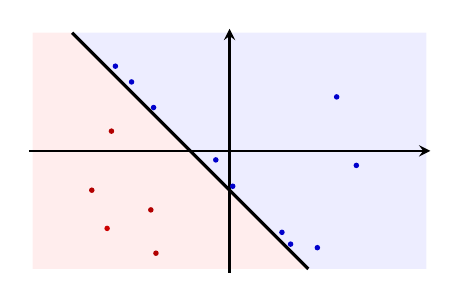
\begin{tikzpicture}[>=stealth, scale=0.5]
        \fill[blue!35!white, opacity = 0.2] (-4, 3) -- (5, 3) -- (5, -3) -- (2, -3)-- cycle;
        \fill[red!35!white, opacity = 0.2] (-4, 3) -- (-5, 3) -- (-5, -3) -- (2, -3)-- cycle;
        \draw[thick, ->] (-5.1, 0)-- (5.1, 0); 
        \draw[thick, ->] (0, -3.1) -- (0, 3.1); 
        \draw[very thick] (-4, 3) -- (2, -3); % node[above right]{\small $H = \{x + y + 1 = 0\}$}; 
        \fill[blue!80!black] (-2.9, 2.15) circle (2pt); 
        \fill[blue!80!black] (-2.49, 1.75) circle (2pt); 
        \fill[blue!80!black] (-1.93, 1.1) circle (2pt); 
        \fill[blue!80!black] (-0.35,-0.23) circle (2pt);
        \fill[blue!80!black] (0.08, -0.9) circle (2pt); 
        \fill[blue!80!black] (1.33, -2.07) circle (2pt);
        \fill[blue!80!black] (1.55, -2.37) circle (2pt); 
        \fill[blue!80!black] (2.23, -2.46) circle (2pt); 
        \fill[blue!80!black] (3.22, -0.37) circle (2pt); 
        \fill[blue!80!black] (2.72, 1.37) circle (2pt); 
        \fill[red!80!black] (-3.11, -1.97) circle (2pt);
        \fill[red!70!black] (-3, 0.5) circle (2pt); 
        \fill[red!70!black] (-3.5, -1) circle (2pt); 
        \fill[red!70!black] (-2, -1.5) circle (2pt); 
        \fill[red!70!black] (-1.87, -2.6) circle (2pt); 
    \end{tikzpicture}
    \caption{Many points near the decision boundary}
    \label{figure:close2decision}
\end{figure}

\end{frame}

%%%%
\begin{frame}
\frametitle{But\ldots data is messy}
If many points close to the decision boundary, likely for newly observed data to appear on ``wrong side'' of decision boundary. Perceptron algorithm gives us nothing to correct for this.

\pause
If ${\bf x}$ is close to decision boundary, we might feel less \emph{confident} in giving the label $h({\bf x})$ that we do. And, if ${\bf x}$ is farther from the boundary, where only one label is seen nearby, more confidence is warranted.

\pause
Also\ldots the immediate change of label across the boundary (a discontinuity in the model) \ldots perhaps not ``natural''?
\end{frame}

\section{Logistic model}

%%%%
\begin{frame}
\frametitle{Incorporating a probability into half-space model}
Instead of only capturing the sign of ${\bf w}\cdot{\bf x} + b$, compose it with the \textbf{logistic function}.    
    \[\sigma(z) = \frac{1}{1+e^{-z}}.\]
\begin{itemize}
    \item $0 < \sigma(z) < 1$ for all $z\in\mathbb R$;
    \item $\lim_{z\to\infty}\sigma(z) = 1$ and $\lim_{z\to-\infty}\sigma(z) = 0$;
    \item $\sigma(0) = 1/2$.
\end{itemize}

\centering
\includegraphics[height=0.3\textheight]{../../Images/logistic_function_graph.png}

\end{frame}

%%%%
\begin{frame}
\frametitle{Logistic model, continued}
    ``Logistic regression'', used for binary classification, as follows.
    
    Find hyperplane $H$, as determined by some ${\bf w}$ and $b$, that fits labeled data well; given new ${\bf x}\in\mathbb R^d$, find $z = {\bf w}\cdot{\bf x}+b$, then compute $\sigma(z)$. 
    \begin{itemize}
        \item (Logistic regression) $\sigma(z)$, the \textit{probability} that the label is $+1$.
    \end{itemize}
    
    \pause
    \begin{enumerate}
        \item If ${\bf w}\cdot{\bf x}+b > 0$ is very large (${\bf x}$ far away from $H$ and on positive side), then  $\sigma(z)$ is very close to $1$.
        \item If ${\bf w}\cdot{\bf x}+b < 0$ has abs.\ value very large (${\bf x}$ far away from $H$ on negative side), then  $\sigma(z)$ very close to $0$.\footnote{Since $-1$ is only other label, high probability of having label $-1$.}
        \item If ${\bf x}$ is contained in $H$ itself, $z=0$ and $\sigma(z) = 0.5$.
    \end{enumerate}
    \pause
    Binary classifier model from logistic regression: $h({\bf x})=1$ if $\sigma({\bf w}\cdot{\bf x}+b) \ge 0.5$, and $h({\bf x})=-1$ otherwise. 
    \begin{itemize}
        \item \textit{Remember that probability (certainty) in the prediction}.
    \end{itemize}

\end{frame}

%%%%
\begin{frame}
\frametitle{Logistic model, continued}
    ``Logistic regression'', used for binary classification, as follows.
    
    Find hyperplane $H$, as determined by some ${\bf w}$ and $b$, that fits labeled data well; given new ${\bf x}\in\mathbb R^d$, find $z = {\bf w}\cdot{\bf x}+b$, then compute $\sigma(z)$. 
    \begin{itemize}
        \item (Logistic regression) $\sigma(z)$, the \textit{probability} that the label is $+1$.
    \end{itemize}
    
    Binary classifier model from logistic regression: $h({\bf x})=1$ if $\sigma({\bf w}\cdot{\bf x}+b) \ge 0.5$, and $h({\bf x})=-1$ otherwise. 
    
    \pause 
    Some rationale for the use of the logistic function $\frac{1}{1+e^{-z}}$ in this process, comes from an inverse direction. 
    \begin{itemize}
        \item If wanting to use \textit{Maximum Likelihood Estimation} to get a binary model, and making some typical simplifying assumptions on conditional probability ($P$), given model parameters, of observing some ${\bf x_i}$ $\leadsto$ $\log\left(\frac{P}{1-P}\right)$ being linear.
    \end{itemize}

\end{frame}
%%%%
\begin{frame}
    \frametitle{How to find ${\bf w}$ and $b$}
    Given $\{\pm1\}$ labeled data, how do we go about finding ${\bf w}$ and $b$ to use in the logistic (regression) model?

    \begin{itemize}
        \item Even if data is linearly separable, Perceptron algorithm does not try to make hyperplane be positioned ``away from'' data (Disadvantage). 
        \item If data is not linearly separable, what should be done?
    \end{itemize}

    Future lectures: Will discuss using \emph{optimization} (calculus-based) to find best parameters $w_1,w_2,\ldots,w_d,b$; process called Gradient Descent. 
    \begin{itemize}
        \item Relevant: relationship between \emph{gradient} of a function and its \emph{directional derivative}.
    \end{itemize}
\end{frame}
%%%%
\begin{frame}
    \frametitle{More messy versus less messy data}
    Could introduce additional parameter (more flexibility).

    For $k > 0$, define \[\sigma_k(z) = \frac{1}{1+e^{-kz}}.\]

    $0 < k < 1$: values of $\sigma_k(z)$ transition from $0$ to $1$ more slowly.\newline 
    $k > 1$: values of $\sigma_k(z)$ transition from $0$ to $1$ more quickly. (think about derivative)

    Hence, if know data has more noise, might use $0 < k < 1$ to decrease measure of confidence in prediction. In contrast, very ``clean'' data, interpretation of the model might benefit from $k>1$.
    
    (\textbf{Left:} graph with $k=5$; \textbf{Right:} applied to points in $\mathbb R^2$)
    \centering
    \begin{multicols}{2}
    \includegraphics[height=0.25\textheight]{../../Images/logistic_function_kis5.png}

    \includegraphics[height=0.25\textheight]{../../Images/logistic_function_appliedtohalfspace.png}
    \end{multicols}
    
\end{frame}

\end{document}